\documentclass[letterpaper,12pt,openright,notitlepage]{report}


\usepackage[T1]{fontenc}
\usepackage[latin1]{inputenc}
\usepackage{indentfirst}        % indenta primeiro par�grafo
\usepackage{graphicx}
\usepackage{subfigure}
\subfigcapmargin = .5cm

\usepackage{fancyref}
\usepackage{textcomp}      % \texttrademark
\usepackage{url}
\usepackage{multirow}
\usepackage{amsmath}
\usepackage{amssymb}
%\ackage{txfonts}
\usepackage{color}
\usepackage[brazil]{babel}    % hiphena��o em portugues
\usepackage{wrapfig}
%Bold vectors and tensors
\usepackage[bold]{hhtensor}
%%\usepackage[round]{natbib}  % cita��es tipo  (nome-ano)
\usepackage{natbib}  % cita��es tipo  [nome-ano]
\usepackage{setspace}

\usepackage[small]{caption}
\setlength{\captionmargin}{20pt}

\renewcommand*\thesection{\arabic{section}}
\setcounter{secnumdepth}{3}
\setcounter{tocdepth}{3}
\usepackage{booktabs}

%-----TIKZ
\usepackage{circuitikz}
\usepackage{ifthen}
\usepackage{tikz}
\usepackage{pgf}
\usepackage{pgffor}
\usepgfmodule{shapes}
\usepgfmodule{plot}
\usetikzlibrary{decorations}
\usetikzlibrary{arrows}
\usetikzlibrary{snakes}
\usetikzlibrary{arrows,positioning} 
\tikzset{
    %Define standard arrow tip
    >=stealth',
    %Define style for boxes
    punkt/.style={
           rectangle,
           rounded corners,
           draw=black, very thick,
           text width=6.5em,
           minimum height=2em,
           text centered},
    % Define arrow style
    pil/.style={
           ->,
           thick,
           shorten <=2pt,
           shorten >=2pt,}
}
%\ctikzset{bipoles/length=1 cm}

%% Hyperlink options
\usepackage{hyperref}
%\hypersetup{colorlinks=true,       % false: boxed links; true: colored links
%	linkcolor=blue,          % color of internal links
%	citecolor=red,        % color of links to bibliography
%	urlcolor=black,
%	bookmarksnumbered=true,
%	pdffitwindow=true, 
%	bookmarks=true,
%    	pdftitle={Controle e Intera��o de F�nons e F�tons em Fibras �pticas de Cristal Fot�nico},    		pdfauthor={Gustavo Silva Wiederhecker}     % author}           % color of external links
%	}         % show bookmarks bar?

%% tamanho do texto e margens
\setlength{\topmargin}{-15pt} % extra vert. space + at the top of header: 23pt
\setlength{\oddsidemargin}{0pt} % extra spc added at the left of odd page: 0pt
\setlength{\evensidemargin}{-12pt} % ext. spc added at the left of even pg: 59pt
\setlength{\textheight}{625pt} % height of the body: 592pt
\setlength{\textwidth}{483pt} % width of the body: 470pt
\setlength{\headheight}{15.6pt} % width of the body: 470pt
\setlength{\footskip}{60pt}
%% Estilo da p�gina corrente e demais p�ginas
\definecolor{Gray}{rgb}{0.5,0.5,0.5}
\usepackage{fancyhdr} 
\pagestyle{fancyplain}
\usepackage{calc} 
%\fancyheadoffset[LE,RO]{\marginparsep+\marginparwidth} 
\renewcommand{\chaptermark}[1]{\markboth{#1}{}} 
\renewcommand{\sectionmark}[1]{\markright{\thesection\ #1}} \fancyhf{}
\fancyhead[LE,RO]{\bfseries\thepage} 
\fancyhead[LO]{\bfseries\rightmark} 
\fancyhead[RE]{\bfseries\leftmark}

\input

%%%% Bold symbol macro for standard LaTeX users
\providecommand{\boldsymbol}[1]{\mbox{\boldmath $#1$}}

%%Figure path
\graphicspath{{figures/}}
%%COMANDOS
\newcommand{\fig}{Fig. }
%% Inicia o texto
\begin{document}

%% Commands
%---------------------------------------------------------------------
%            SHORTCUTS USED IN THE TEXT
%---------------------------------------------------------------------
% CUSTOM SHORTCUTS
\newcommand{\neff}{n_\text{eff}}
\newcommand{\ml}{Matlab\textsuperscript{\textregistered} }
\newcommand{\cm}{Comsol\textsuperscript{\textregistered} }
\newcommand{\sinn}{Si$_3$N$_4$\text{ }}
\newcommand{\sio}{SiO$_2$\text{ }}
%
%\newcommand*{\eps0}{ \epsilon_0 }
%\newcommand{\mu0}{\mu$_0$}

%------------------------------------------
%vector calculus
\newcommand{\divg}[1]{\nabla \cdot \vec{#1}}
\newcommand{\rot}[1]{\nabla \times \vec{#1}}

%------------------------------------------
%time derivatives
\newcommand{\dpt}[1]{\frac{\partial \vec{#1}}{\partial t}}
\newcommand{\dt}[1]{\frac{d \vec{#1}}{d t}}

%------------------------------------------
%			TWO PORT NETWORK
%------------------------------------------
\newcommand{\tpn}[2]{
	\begin{circuitikz}[scale=1]
		\node (Xi) at (0.7,0.7) {$V_1$};
		\node (Xf) at (3.7,0.7) {$V_2$};
		\draw [semithick,->] (Xi) -- (0.1,0.1);
		\draw [semithick,->] (Xf) -- (3.1,0.1);
		\draw
			to [generic, o-o, l_=$#1$] ++(2,0)
			(2,0) to [short,o-o] ++(1,0)
			(2,0) to [generic, o-o, l=$#2$] ++(0,-2)
			node[ground] {}
			;
	\end{circuitikz}
}

\newcommand{\tpn}[2]{
	\begin{circuitikz}[scale=1]
		\node (Xi) at (0.7,0.7) {$V_1$};
		\node (Xf) at (3.7,0.7) {$V_2$};
		\draw [semithick,->] (Xi) -- (0.1,0.1);
		\draw [semithick,->] (Xf) -- (3.1,0.1);
		\draw
			to [generic, o-o, l_=$#1$] ++(2,0)
			(2,0) to [short,o-o] ++(1,0)
			(2,0) to [generic, o-o, l=$#2$] ++(0,-2)
			node[ground] {}
			;
	\end{circuitikz}
}	
%------------------------------------------
%			PHASOR DIAGRAM
%------------------------------------------
\newcommand{\Gitter}[4]{
    \draw[very thin,color=gray] (#1,#3) grid (#2,#4);
}
\newcommand{\Koordinatenkreuz}[6]{
    \draw[->, >=latex, color=green!50!black] (#1,0) -- (#2,0) node[right] {#5};
    \draw[->, >=latex, color=green!50!black] (0,#3) -- (0,#4) node[left] {#6};
}
\newcommand{\KoordinatenkreuzOhneLabelsVerschobenKeinPfeil}[5]{
    \draw[-] (#1,0) -- (#2,0);
    \draw[-] (#5,#3) -- (#5,#4);

}
\newcommand{\ZeigerdiagrammText}[4]{
\begin{tikzpicture}[scale=.72, samples=100, >=latex]

    \def\Alpha{#1}
    \def\Phase{#2}
    \def\AmplitudeSpannung{#3}
    \def\AmplitudeStrom{#4}
    \def\SpannungsWert{{\AmplitudeSpannung*sin(\Alpha)}}
    \def\StromWert{{\AmplitudeStrom*sin(\Alpha+\Phase)}}
    %%%%%%%%%%%%%%%%%%%%%%%%%%%%%%%%%%%%%%%%%%%%%%%%%%%%%%%%%%
    \def\FarbeSpannung{blue!90!white}
    \def\FarbeStrom{red!90!white}
    \def\FarbeWinkelZeichnung{green}
    %%%%%%%%%%%%%%%%%%%%%%%%%%%%%%%%%%%%%%%%%%%%%%%%%%%%%%%%%%
    \def\Beta{\Alpha+\Phase}
    \def\AlphaRad{\Alpha*3.141592654/180}
    \def\PhaseRad{\Phase*3.141592654/180}
    %%%%%%%%%%%%%%%%%%%%%%%%%%%%%%%%%%%%%%%%%%%%%%%%%%%%%%%%%%
    \Gitter{-.1}{7.1}{-3.1}{3.1}
    \Koordinatenkreuz{-.2}{7.3}{-3.2}{3.3}{$\omega t$}{}
    \draw (1.570795,0) node[below]{$\frac{\pi}{2}$};
    \draw (3.14159,0) node[below]{${\pi}$};
    \draw (4.71238898,0) node[below]{$\frac{3\pi}{2}$};
    \draw (6.283185307,0) node[below]{${2\pi}$};
    \draw (-4,0) circle (3cm);
    \KoordinatenkreuzOhneLabelsVerschobenKeinPfeil{-7.2}{-.8}{-3.6}{3.6}{-4}
    %%%%%%%%%%%%%%%%%%%%%%%%%%%%%%%%%%%%%%%%%%%%%%%%%%%%%%%%%%

    % voltage
    \draw[color=\FarbeSpannung, very thick] plot[id=voltage, domain=0:7] function{\AmplitudeSpannung*sin(x)} node[right] {$U(t)$};
    % voltage circle
    \draw[color=\FarbeSpannung, loosely dashed] (-4,0) circle (\AmplitudeSpannung cm);
    % angle
    \draw[color=\FarbeWinkelZeichnung!50!black, thick] (\AlphaRad, \SpannungsWert)--(\AlphaRad,\StromWert) node[below=18pt] {$\alpha$};
    % angle in the circle
    \filldraw[fill=\FarbeWinkelZeichnung!20,draw=\FarbeWinkelZeichnung!50!black] (-4,0) -- (-3,0) arc (0:\Alpha:1) -- cycle node[right] {$\alpha$};
    % voltage pointer
    \draw[<-,color=\FarbeSpannung, very thick] (\Alpha:\AmplitudeSpannung)++(-4,0) --(-4,0);
    \draw[color=\FarbeSpannung,  dashed] (\Alpha:\AmplitudeSpannung)++(-4,0) -- (\AlphaRad,\SpannungsWert);
    % current
    \draw[color=\FarbeStrom, very thick] plot[id=current, domain=0:7] function{\AmplitudeStrom*sin(x+\PhaseRad)} node[right] {$I(t)$};		
    % current circle
    \draw[color=\FarbeStrom, loosely dashed]    (-4,0) circle (\AmplitudeStrom cm);
    % current pointer
    \draw[<-,color=\FarbeStrom, very thick] (\Beta:\AmplitudeStrom)++(-4,0) --(-4,0);
    \draw[color=\FarbeStrom,  dashed](\Beta:\AmplitudeStrom)++(-4,0) -- (\AlphaRad,\StromWert);
    % phase difference
    \ifthenelse{\Phase<0}{
        \draw[snake=brace] (pi/2 ,3.3)--(pi/2-\PhaseRad ,3.3) node[above=7pt, left=10pt] {$\phi$};
    }
    {
        \draw[snake=brace] (pi/2-\PhaseRad ,3.3)--(pi/2 ,3.3) node[above=7pt, left=10pt] {$\phi$};
    }
    % angular velocity \omega
    \draw[->, xshift=-4cm]  (120:2.4cm) arc (120:170:2) node[below] {$\omega$};
\end{tikzpicture}
}
%% Abrevia figuras e tabelas
\def\figurename{Fig.}
\def\tablename{Tab.}

%% P�gina de rosto
%%
%% ********** P�gina de Rosto
%%

%% n�o numerar a p�gina
\thispagestyle{empty}
%unicamp logo
\begin{figure}
\begin{center}

\includegraphics[width=3cm]{logo_unicamp}
\end{center}
\end{figure}

\begin{center}
{\Large \textbf{Circuitos de Corrente Alternada}}\\ \vspace{2ex}

\vspace{0.6in}
{\large Hugo L. Fragnito\\}
{\large Gustavo S. Wiederhecker\\}
\vspace{1.2in}
Campinas, SP \\
2011
\end{center}




% Lista de conte�do (sum�rio)
\def\contentsname{Sum�rio}
\tableofcontents

%%% line spacing
\onehalfspacing
% Cap. 1 - Introdu��o
%\include{F429_cap1}
%\include{F429_cap2}
%AC - Diodo semicondutor
%----------------------------------
\chapter{\label{sec:filtros} Experimento I - Filtros}
\begin{figure}[hbt]
\begin{center}
\begin{circuitikz}[scale=1]
		\draw
			(0,0) node[ground] {}
			to [sinusoidal voltage source, o-o, l=$\epsilon(t)$] ++(0,2)
			to [generic, o-o, l=$Z_g$] ++(2,0)
			to [generic, o-o, l=$Z_1$] ++(2,0)
			(4,2) to [short,o-o] ++(1,0)
			(4,2) to [generic, o-o, l=$Z_2$] ++(0,-2)
			node[ground] {}
			;
		%Description of subparts
		\draw [decorate,decoration={brace,amplitude=8pt},
					xshift=0pt, yshift=0pt]
					(2,-1) -- (-0.5,-1)
					node[black,midway,yshift=-20pt]
						{Gerador AC};
		\draw [decorate,decoration={brace,amplitude=8pt},
					xshift=0pt, yshift=0pt]
					(5,-1) -- (2.1,-1)
					node[black,right,yshift=-20pt]
						{Circuito de duas portas};	
	\end{circuitikz}
  \caption{Generic two-port circuit setup. $Z_g$ represents the internal impedance of the AC generators, $Z_1,Z_2$ are any generic linear circuit components. The arrows $V_1$ and $V_2$ indicate where we connect  oscilloscope channels to the circuit. }
  \end{center}
  \label{fig:generic_two_port}
\end{figure}
%----------------------------------
%-------OBJETIVOS------------------
%----------------------------------
\subsection{Objetivos}
Entender o papel ...
\subsection{Introdu��o}
Introduction goes here...
\subsubsection{Diodo demodulador ou detector}
% \begin{wrapfigure}{r}{0.5\textwidth}
%  \vspace{-20pt}
%  \begin{center}
%    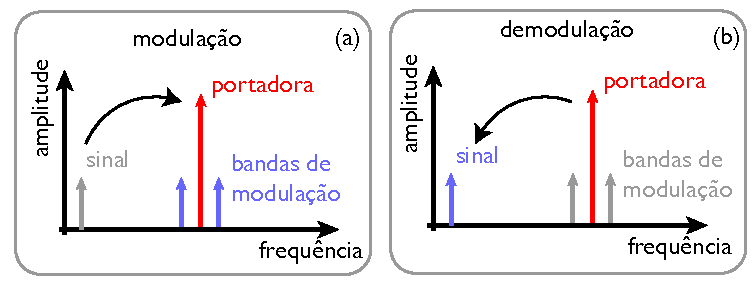
\includegraphics[width=0.5\textwidth]{mod_e_demod}
%  \end{center}
%   \vspace{-20pt}
%  \caption{Princ�pio de modula��o de demodula��o de um sinal.}
%\end{wrapfigure}
%----------------------------------
%-------PREPARA��O-----------------
%----------------------------------
\subsection{Prepara��o}
\begin{enumerate}
\item Calcule a fun��o... 
\end{enumerate}
%----------------------------------
%-------MATERIAL-----------------
%----------------------------------

%----------------------------------
%----------Roteiro-----------------
%----------------------------------
\subsection{Roteiro A - Circuito RC}
\begin{figure}
\centering
\subfigure[Circuito RC com tens�o de sa�da medida no capacitor, $V_2=\frac{1}{j\omega C}i$]{
\tpnc{resistor}{R}{capacitor}{C}}
\subfigure[Circuito RC com tens�o de sa�da medida no resistor, $V_2=R i$]{
\tpnc{capacitor}{C}{resistor}{R}}
\end{figure}


\subsubsection*{Material}
\begin{itemize}
\item Diodo de  sil�cio.
\end{itemize}
\subsubsection*{Caracteriza��o do circuito LC}
\subsection{Roteiro B - Circuito RLC}
Nesta etapa desejamos estudar experimentalmente o fen�meno de resson�ncia em circuitos RLC. Iremos determinar a resposta em frequ�ncia deste circuito (amplitude e fase) e investigar suas principais caracter�sticas, frequ�ncia de resson�ncia, largura de banda e pot�ncia dissipada.
\begin{figure}[hb]
\subfigure[ ]{
\begin{circuitikz}[scale=.8]
		\node (Xi) at (0.7,0.7) {$V_1$};
		\node (Xf) at (5.7,0.7) {$V_2$};
		\draw [semithick,->] (Xi) -- (0.1,0.1);
		\draw [semithick,->] (Xf) -- (5.1,0.1);
		\draw	to [inductor, o-o, l_=L] ++(2,0)
				to [capacitor, o-o, l_=C] ++(2,0)
				(4,0) to [short,o-o] ++(1,0)
				(4,0) to [resistor, o-o, l=R] ++(0,-2)
				node[ground] {};
	\end{circuitikz}}
\subfigure[ ]{
\begin{circuitikz}[scale=.8]
		\node (Xi) at (0.7,0.7) {$V_1$};
		\node (Xf) at (5.7,0.7) {$V_2$};
		\draw [semithick,->] (Xi) -- (0.1,0.1);
		\draw [semithick,->] (Xf) -- (5.1,0.1);
		\draw	to [resistor, o-o, l_=R] ++(2,0)
				to [capacitor, o-o, l_=C] ++(2,0)
				(4,0) to [short,o-o] ++(1,0)
				(4,0) to [inductor, o-o, l=L] ++(0,-2)
				node[ground] {};
	\end{circuitikz}}
\subfigure[ ]{
\begin{circuitikz}[scale=.8]
		\node (Xi) at (0.7,0.7) {$V_1$};
		\node (Xf) at (5.7,0.7) {$V_2$};
		\draw [semithick,->] (Xi) -- (0.1,0.1);
		\draw [semithick,->] (Xf) -- (5.1,0.1);
		\draw	to [inductor, o-o, l_=L] ++(2,0)
				to [resistor, o-o, l_=R] ++(2,0)
				(4,0) to [short,o-o] ++(1,0)
				(4,0) to [capacitor, o-o, l=C] ++(0,-2)
				node[ground] {};
	\end{circuitikz}}
	\caption{\textbf{Diferentes configura��es de um filtro RLC}. }
\end{figure}
\subsubsection*{Caracteriza��o da curva IV do diodo}
%----------------------------------
%----------Relatorio-----------------
%----------------------------------
\subsection{Relat�rio}


\newpage
\chapter{\label{sec:transientes} Experimento II - Transientes}

%----------------------------------
%-------OBJETIVOS------------------
%----------------------------------
\subsection{Objetivos}
Entender o papel ...
\subsection{Introdu��o}
Introduction goes here...
\subsubsection{Diodo demodulador ou detector}
% \begin{wrapfigure}{r}{0.5\textwidth}
%  \vspace{-20pt}
%  \begin{center}
%    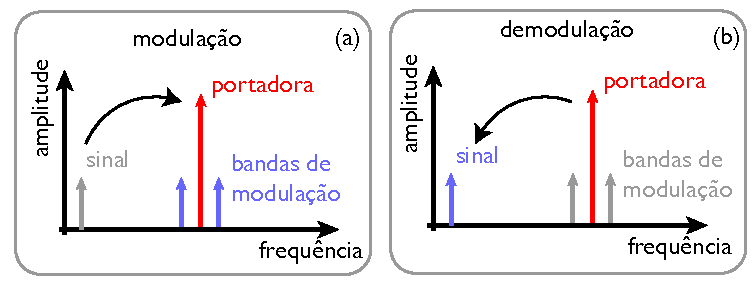
\includegraphics[width=0.5\textwidth]{mod_e_demod}
%  \end{center}
%   \vspace{-20pt}
%  \caption{Princ�pio de modula��o de demodula��o de um sinal.}
%\end{wrapfigure}
%----------------------------------
%-------PREPARA��O-----------------
%----------------------------------
\subsection{Prepara��o}
\begin{enumerate}
\item Calcule a fun��o... 
\end{enumerate}
%----------------------------------
%-------MATERIAL-----------------
%----------------------------------

%----------------------------------
%----------Roteiro-----------------
%----------------------------------
\subsection{Roteiro A - Circuito RC}
\subsubsection*{Material}
\begin{itemize}
\item Diodo de  sil�cio.
\end{itemize}
\subsubsection*{Caracteriza��o do circuito LC}
\subsection{Roteiro B - Circuito RLC}
\subsubsection*{Caracteriza��o da curva IV do diodo}
%----------------------------------
%----------Relatorio-----------------
%----------------------------------
\subsection{Relat�rio}


%----------------------------------
\newpage
\section{\label{sec:linhas_de_transmissao}Diodo semicondutor e receptor AM}
\begin{figure}[htbp]
\begin{center}
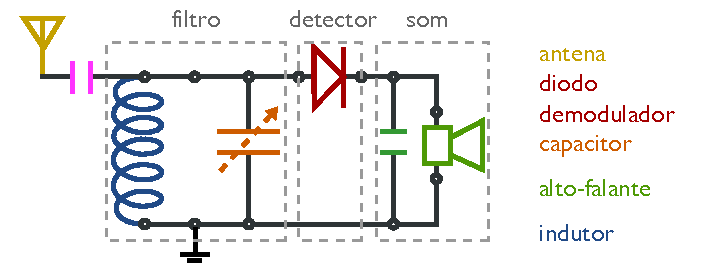
\includegraphics[width=0.7\textwidth]{diagrama_radio_am}
\caption{\textbf{Diagrama de um receptor de  r�dio AM}.}
\label{fig:radio_am}
\end{center}
\end{figure}
\subsection*{Objetivos}
Entender o papel dos componentes de um receptor AM (\textit{amplitude modulation}) e montar um receptor de ondas AM . Para tanto iremos estudar experimentalmente a curva IV (corrente-tens�o) de um diodo e tamb�m a resposta do filtro de sintonia.
\subsection*{Introdu��o}
\subsubsection*{Diodo demodulador ou detector}
 \begin{wrapfigure}{r}{0.5\textwidth}
  \vspace{-20pt}
  \begin{center}
    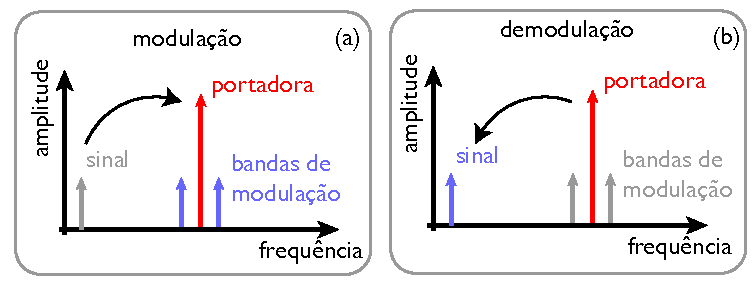
\includegraphics[width=0.5\textwidth]{mod_e_demod}
  \end{center}
   \vspace{-20pt}
  \caption{Princ�pio de modula��o de demodula��o de um sinal.}
\end{wrapfigure}
A transmiss�o de informa��o por ondas de r�dio � feita atrav�s da modula��o de uma onda portadora (\textit{carrier}) de alta frequ�ncia, $0.8<f_c<1.1$ MHz para AM (\textit{amplitude modulation}) ou $88<f_c<105$ MHz para FM (\textit{frequency modulation}), com o sinal de audio que deseja ser transmitido, tipicamente com frequ�ncia entre 20 Hz e 10 KHz. Na figura \ref{fig:am_fm} ilustramos estes dois tipos de modula��o.  A modula��o permite que a a informa��o seja transmitida atrav�s de uma portadora em uma frequ�ncia mais alta que a frequ�ncia do sinal; na frequ�ncia  da portadora espera-se melhores caracter�sticas de propaga��o, i.e., menor atenua��o, dispers�o. Tamb�m � poss�vel utilizar outro tipo de onda, por exemplo, ondas eletromagn�ticas para transmitir a informa��o, por exemplo, r�dios AM exploram a alta refletividade da ionosfera para para transmitir  ondas eletromagn�ticas por longas dist�ncias.
\begin{figure}[htbp]
\begin{center}
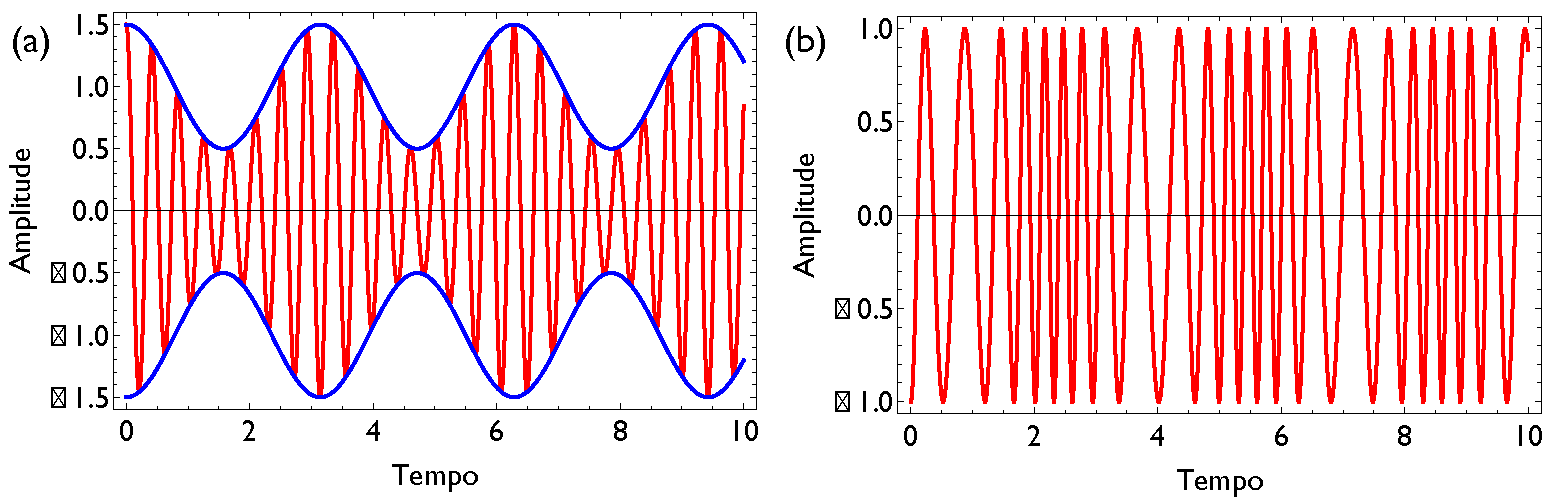
\includegraphics[width=0.9\textwidth]{FM}
\caption{\textbf{Modula��o de ondas}. (a) Modula��o de amplitude (AM), $A(t)=(1+\delta \cos[\Omega t])\cos[\omega_c t]$. (b) Modula��o de frequ�ncia (FM), $A(t)=\cos[\omega_c t+\delta \cos[\Omega t]]$}
\label{fig:am_fm}
\end{center}
\end{figure}

\subsubsection*{Antena}
Quando uma onda eletromagn�tica com frequ�ncia $f_c$ e comprimento de onda $\lambda=c/f_c$  incide sobre uma antena, um dipolo oscilante � induzido na antena. O dipolo induzio gera uma corrente no circuito no qual a antena est� conectada. Para que a excita��o do dipolo seja eficiente
na mesma, � importante que o comprimento da antena $L$ seja, aproximadamente,  uma fra��o inteira do comprimento de onda. No nosso laborat�rio $L\approx17$ m, aproximadamente, $\lambda/10$ para as frequ�ncias de r�dio AM. 
\subsubsection*{Filtro ressonante}
Como existem diversas esta��es de r�dio AM, � necess�rio tamb�m filtrar o sinal recebido pela antena.  Para tanto utilizaremos um circuito LC em paralelo, como mostra a Fig. \ref{fig:radio_am}, este filtro funciona como um passa-banda, selecione a esta��o de r�dio que desejamos ouvir.
\subsubsection*{Diodo demodulador ou detector}
 \begin{wrapfigure}{r}{0.3\textwidth}
  \vspace{-40pt}
  \begin{center}
    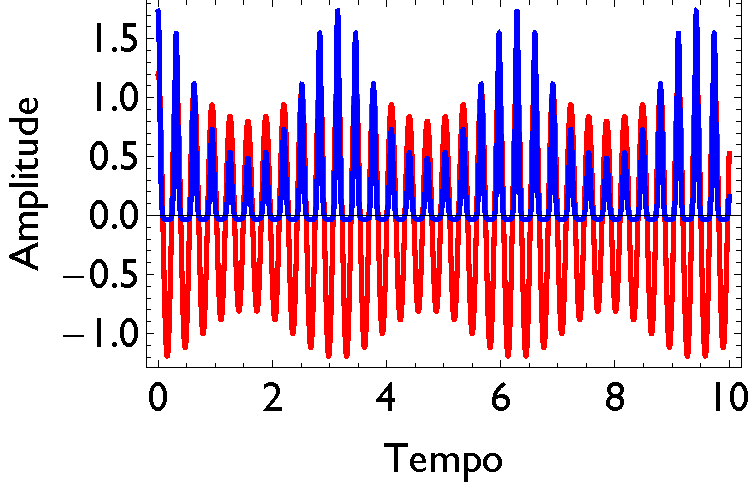
\includegraphics[width=0.3\textwidth]{diode_demodulation}
  \end{center}
   \vspace{-20pt}
  \caption{\textbf{Demodula��o por um diodo}}
\end{wrapfigure}

 Da mesma forma que modulamos a portadora para transmitir o sinal � necess�rio demodular a onda recebida para podermos escut�-la no alto-falante. Este � o papel do diodo neste circuito, devido a sua curva IV n�o-linear este componente recupera o sinal de audio que foi modulado na onda portadora.
 
\subsection*{Prepara��o}
\begin{enumerate}
\item Calcule a fun��o de trasfer�ncia $H(\omega)$ do filtro LC mostrado na figura \ref{fig:radio_am}. Mostre que a transmit�ncia ($|H|^2$) � dada por  $T(\omega)=\frac{L^2 \omega ^4 C_{in}^2}{\left(L \omega ^2 \left(C_{in}+C_v\right)-1\right){}^2}$. 
\item Qual � a frequ�ncia de resson�ncia deste filtro? 
\item Assumindo que o indutor possui $L=62\mu$H e o capacitor vari�vel pode variar entre $30\text{ pf}<C_v<350\text{ pf}$, calcule a faixa de frequ�ncias que este filtro poder� sintonizar. Descubra na internet quais r�dios de Campinas est�o nesta faixa.
\item Assuma que  a curva IV de um diodo pode ser aproximada pela express�o $i(t)=a_1 v(t)+a_2 v^2(t)$, onde $a_1$ e $a_2$ s�o constantes. Calcule a corrente quando a tens�o for na forma $v(t)=v_0(1+m(t))\cos[\omega_c t]$. Mostre que existe um termo proporcional � $m(t)$. Pense no  que acontece com os demais termos ao passar pelo capacitor do alto-falante?
\end{enumerate}
\subsection*{Material}
\begin{itemize}
\item Diodo de  sil�cio.
\item Diodo de germ�nio tipo Schotky (Nunca aplicar um sinal do gerador neste diodo, ele � sens�vel e pode queimar!).
\item Indutor e capacitor sintoniz�vel ( $30\text{ pf}<C_v<350\text{ pf}$) (Estes componentes j� est�o montados!).
\item Resistores: 1k $\Omega$.
\end{itemize}
\subsection*{Roteiro}
\subsubsection*{Caracteriza��o do circuito LC}
 \begin{wrapfigure}{r}{0.3\textwidth}
  \vspace{-30pt}
  \begin{center}
    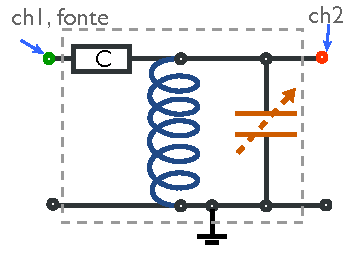
\includegraphics[width=0.3\textwidth]{tuning_lc}
  \end{center}
   \vspace{-20pt}
  \caption{\textbf{Esquema do circuito para caracterizar o filtro LC}. Utilize o gerador de fun��es no canal 1.}
  \label{fig:tuning}
\end{wrapfigure}
Para caracterizar o filtro iremos utilizar a montagem da Fig. \ref{fig:tuning}. Acople o sinal do gerador no terminal \textbf{verde} do filtro, me�a o sinal de sa�da no terminal \textbf{vermelho}. Estime a frequ�ncia de resson�ncia esperada e depois encontre-a experimentalmente para 4 diferentes posi��es das placas do capacitor sintoniz�vel. Com a maior capacit�ncia poss�vel, me�a 10 pontos das amplitudes $V_{pp1}/V_{pp2}$ na faixa de 50 KHz em torno da resson�ncia. No relat�rio estime a largura de banda do filtro.

\subsubsection*{Caracteriza��o da curva IV do diodo}

Em teoria poder�amos medir a curva IV de um diodo simplesmente introduzindo um resistor $R$ em s�rie com o diodo. A queda de tens�o  no resistor seria proporcional � corrente, portanto $I=V_R/R$. Para obter $V_D$ basta medirmos a queda de tens�o no diodo. Contudo, no  laborat�rio precisamos conectar o canal 1 do oscilosc�pio entre os terminais do diodo e o canal 2 entre os terminais de resistor. Como o terra de ambos canais � o mesmo, tal conex�o implicaria no resistor (ou o diodo)  em curto-circuito, portanto a queda de tens�o medida seria nula. Para resolver este problema de aterramento iremos explorar o transformador de tens�o pois neste o enrolamento prim�rio (conectado � rede el�trica) est� isolado do secund�rio (conectado ao circuito), consequentemente podemos impor um ponto de terra entre o resistor e o diodo, como ilustra a Fig. \ref{fig:diodo_iv}\footnote{Note que se fiz�ssemos esta conex�o utilizando o gerador sem o transformador, o resistor conectado ao terminal central do indutor estaria em curto-circuito.}. Como invertemos o sentido que estamos medindo a tens�o no resistor, � tamb�m necess�rio \textbf{inverter} o sinal do canal 2 do oscilosc�pio.

\begin{enumerate}
\item Monte o circuito da  Fig. \ref{fig:diodo_iv}.
\item No modo $YT$ do oscilosc�pio centralize ambas (canais 1 e 2) ondas em $Y=0$ e e grave no seu cart�o de mem�ria.
\item No modo $XY$ salve 2 vers�es da curva IV, uma em que a curva toda possa ser visualizada (ajuste as escalas horizontais e vertical) e outra em que a origem (pr�ximo de $V_R=0, V_D=0$) esteja ampliada.
\end{enumerate}

No seu relat�rio inclua as tr�s curvas. Para as curvas IV indique a escala vertical como corrente em mA e o eixo horizontal em V.
Extraia destas curvas a corrente de satura��o e tamb�m a inclina��o da curva $dI/dV$, para polariza��o reversa ($V<0$) e tr�s pontos distintos para polariza��o direta ($V>0$). Calcule a resist�ncia diferencial nestes pontos $R=(dI/dV)^{-1}$
 \begin{wrapfigure}{r}{0.5\textwidth}
  \vspace{0pt}
  \begin{center}
    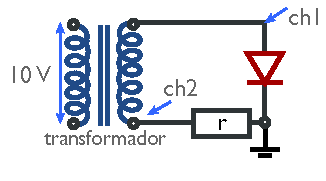
\includegraphics[width=0.5\textwidth]{diodo_iv}
  \end{center}
   \vspace{-20pt}
  \caption{\textbf{Esquema do circuito para caracterizar a curva IV}. Utilize o transformador de $9$ V de sa�da e $R=1K\Omega$ e um diodo de sil�cio \textbf{(encapsulamento preto!)}.}
  \label{fig:diodo_iv}
\end{wrapfigure}
\subsubsection*{Ouvindo o r�dio}
Chegou finalmente o momento de ouvirmos alguma m�sica (ou not�cias). Monte o circuito da Fig. \ref{fig:radio_am} utilizando como detetor o diodo schotky. A motivo de usarmos este diodo, ao inv�s do diodo de sil�cio,  � que a tens�o cr�tica na qual este diodo deixa passar corrente ($V_0\approx 30$ mV) � muito menor que o diodo de sil�cio ($V_0\approx 700$ mV). Isto o torna ideal para demodular sinais de pequena amplitude, como o que recebemos da antena. Muito cuidado com este diodo pois ele � sens�vel e n�o temos muitos sobrando. Descreva no relat�rio quais r�dios voc� consegui sintonizar. Em Campinas existem duas r�dios nesta faixa de frequ�ncias, a r�dio Central e a r�dio Bandeirantes

%----------------------------------
\newpage
\section{\label{sec:linhas_de_transmissao}Linhas de transmiss�o}

\subsection*{Objetivos}
Estudar experimentalmente o funcionamento de uma linha de transmiss�o e determinar a imped�ncia caracter�stica, o coeficiente de reflex�o e a velocidade de propaga��o de pulsos.
\subsection*{Material}
\begin{itemize}
\item Cabo coaxial RG-58U (ou cabo de par tran�ado ou cabo de antena de TV) de comprimento (conhecido) x $\approx$ 100 m.
\item Acoplador BNC "T"
\item Gerador de pulsos de dura��o menor que 1 $\mu$s. No lugar de um gerador de pulsos pode ser utilizado um gerador de fun��es de pelo menos 2 MHz com duty-cycle vari�vel (por exemplo, o Tektronix CFG 250): Selecione o modo de onda quadrada e ajuste o duty-cycle ao m�nimo.
\item Oscilosc�pio de pelo menos 50 MHz
\item Resistores: 10, 22, 33, 47, 56, 75, 100, 220, 330 e 470 $\Omega$.
\end{itemize}

\subsection*{Roteiro}

\begin{figure}[htbp]
\begin{center}
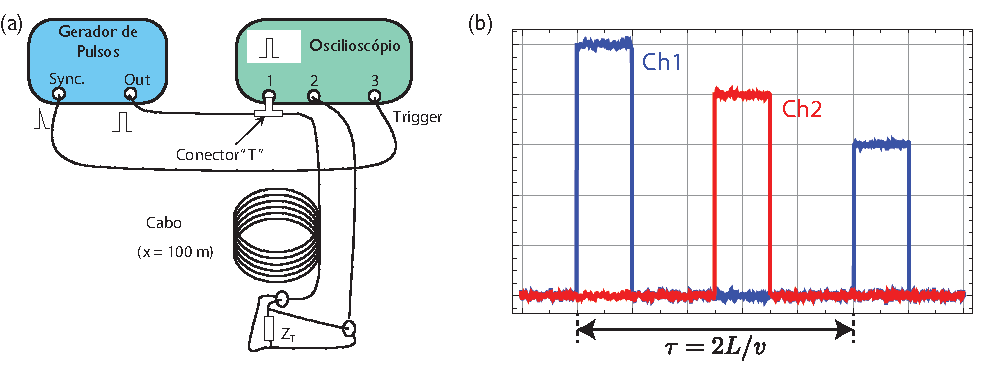
\includegraphics[scale=1]{transmission_line1}
\caption{a) Esquema de montagem. b) Pulsos observados no oscilosc�pio quando a linha n�o � terminada ($Z_T=\infty$). }
\label{fig:transmission_line}
\end{center}
\end{figure}

\begin{enumerate}
\item Monte o circuito da figura \ref{fig:transmission_line}a). Ajuste a taxa de repeti��o de pulsos em 500 kHz ou menos e a dura��o do pulso entre 100 e 200 ns. Se n�o tiver um gerador de pulsos, pode utilizadar um gerador de fun��es de 2 MHz com duty-cycle vari�vel (por exemplo, o Tektronix CFG 250): ajuste a frequ�ncia em 1 MHz ou menos; selecione o modo de onda quadrada e ajuste o duty-cycle ao m�nimo. No canal 1 do oscilosc�pio ver� o pulso de entrada   e o refletido  . No canal 2 ver� o pulso no fim da linha   (utilize um cabo curto para ligar $Z_T$ ao canal 2). Para uma melhor estabilidade, utilize o sinal de sincronismo do gerador para disparar o oscilosc�pio pelo canal 3 (o sincronismo com o canal 1 tamb�m funciona bem).

\item Me�a o atraso temporal entre o pulso lan�ado e o refletido e determine a velocidade de propaga��o do pulso. (Utilize o comprimento medido, L, escrito na etiqueta do cabo). Compare este resultado com a velocidade a luz! Quanto � o �ndice de refra��o, n, do diel�trico do cabo? Quanto � a constante diel�trica relativa ($\epsilon_r\equiv=\epsilon/\epsilon_0=n^2$). Com este valor de $n$ voc� poderia medir o comprimento de um cabo id�ntico com L desconhecido.

\item Para valores fixos de amplitude ($V_0 = V^{+}(0)$), dura��o e periodicidade do pulso, me�a a amplitude do pulso de retorno $V_r = V^{-}(2L)$ para v�rios valores de $Z_T$ (utilize resistores fixos, n�o a resist�ncia de d�cadas) entre 10 e 330 $\Omega$, inclusive para o caso $Z_T = 0$ (curto circuito) e $Z_T = \infty$ (circuito aberto). Construa uma tabela com os valores de $Z_T$ e do coeficiente de reflex�o normalizado $\rho_n = V_R/V_0$. O pulso refletido se deve anular quando $Z_T = Z_0$. Determine, assim, $Z_0$ experimentalmente. Utilize resistores em s�rie e/ou em paralelo para obter mais valores de $Z_T$. Por exemplo, para obter 75 $\Omega$ (o valor nominal de $Z_0$ do cabo coaxial de TV a cabo) utilize dois de 150 $\Omega$ em paralelo.

\item Aumente a dura��o do pulso gradualmente at� alguns microssegundos e veja se entende o que acontece no oscilosc�pio. 

\item Se $Z_T = \infty$ o pulso refletido tem amplitude $V_0 \exp(-\alpha L)$. Utilizando este fato, determine o coeficiente de atenua��o ? (expresse o resultado em dB/100m: $\alpha[\text{dB}/100\text{m}] = 10^3 \alpha[\text{m}^{-1}]/\log(10)  \approx 434 \alpha[\text{m}^{-1}]$).

\item Me�a o atraso e a amplitude entre o pulso lan�ado e o pulso refletido (com $Z_T=0$) para  um cabo diferente do utilizado nos itens anteriores . Dispomos de cabos de rede de par tran�ado, ou UTP, cabo coaxial para TV a cabo e cabo coaxial de instrumenta��o RG-58 --- veja a Fig. \ref{fig:exemplo_cabos}. Calcule o valor do �ndice de refra��o  $n$ e $\alpha$) Compare os coeficientes de atenua��o obtidos para os diferentes cabos (quanto menor � $\alpha$, melhor sua qualidade). 
\end{enumerate}

\begin{figure}[htbp]
\begin{center}
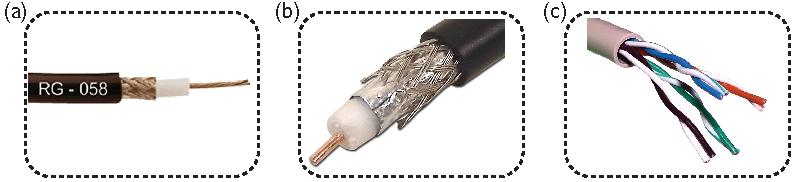
\includegraphics[scale=1]{transmission_line1-02}
\caption{(a) Cabo de instrumenta��o (RG-58). (b) Cabo de TV a cabo (CATV: Cable TV). (c) Cabo de par tran�ado para redes de inform�tica (UTP - Unshielded Twisted Pair). }
\label{fig:exemplo_cabos}
\end{center}
\end{figure}

%----------------------------------
\newpage
\section{\label{sec:interferometros}Interfer�metros}
\begin{figure}[htbp]
\begin{center}
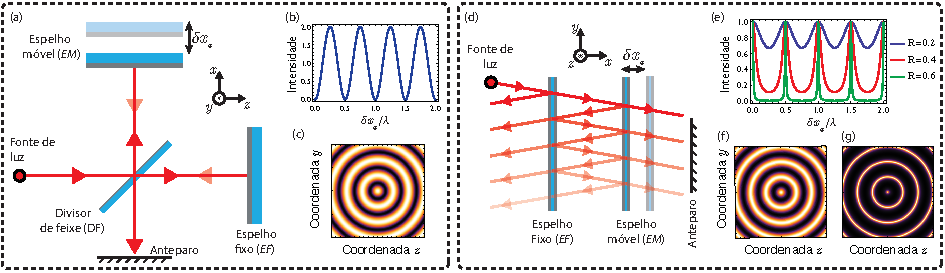
\includegraphics{interferometers}
\caption{\textbf{Diagrama e exemplos de duas importantes classes de interfer�metros �pticos.} (a,d) Esquema de um interfer�metro de Michelson (a) e de Fabry-Perot (d). O espelho $EM$ est� preso a um parafuso microm�trico e pode ter sua posi��o controlada com precis�o submicrom�trica. (b,e) Intensidade �ptica observada em um ponto do anteparo quando varia-se a posi��o do espelho. Em (e), as diferentes curvas representam intefer�metros Fabry-Perot montados com espelhos de diferentes refletivdades $R$.  (c,f,g) Distribui��o transversal de intensidade observada  no anteparo quando o interfer�metros est�o alinhados.}
\label{fig:interferometro}
\end{center}
\end{figure}
\subsection*{Objetivos}
Entender os princ�pios e aplica��es de interfer�metros �pticos, utilizando-los para medir deslocamentos nanom�tricos e para desvendar o conte�do espectral de fontes luminosas. Este roteiro explora os dois tipos de interfer�metro mostrados na \fig\ref{fig:interferometro}. 
\subsection*{Introdu��o}
\subsubsection*{Interfer�ncia entre ondas}
 \begin{wrapfigure}{r}{0.5\textwidth}
  \vspace{-20pt}
  \begin{center}
    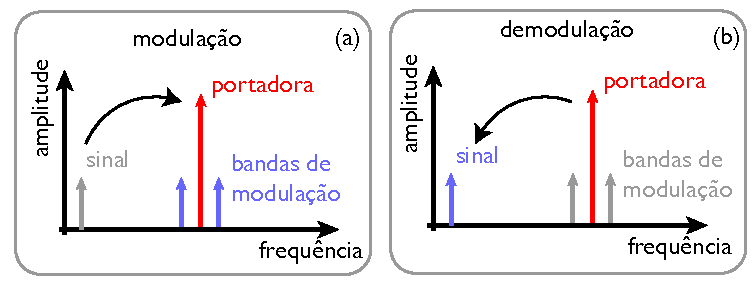
\includegraphics[width=0.5\textwidth]{mod_e_demod}
  \end{center}
   \vspace{-20pt}
  \caption{Princ�pio de modula��o de demodula��o de um sinal.}
\end{wrapfigure}
A interfer�ncia � um fen�meno comumente observado quando trata-se de ondas, o caso eletromagn�tico (ou �ptico) � apenas um exemplo. O fen�meno de intefer�ncia tem como base o princ�pio da superposi��o, segundo o qual o campo el�trico (ou magn�tico) resultante em um dado ponto do espa�o � a soma linear entre o campo gerado por todas as fontes existentes no universo\footnote{� bastante intrigante pensar nisto. Imagine a sua posi��o espacial neste momento, existem fontes de campos eletromagn�ticos distribu�dos por todo o universo, algumas a bilh�es de anos luz de dist�ncia, outras t�o pr�ximas quanto seu telefone celular, todas contribuindo para o campo el�trico total na sua posi��o atual.}. Em favor da simplicidade, consideremos o campo total gerado por duas fontes,
\begin{equation}
\vec{E}(\vec{r},t)=\vec{E}_1(\vec{r},t)+\vec{E}_2(\vec{r},t)
\end{equation}
Para simplicar ainda mais o problema vamos considerar uma situa��o pr�xima � dos nossos interfer�metros, vamos assumir a os campos $\vec{E}_1,\vec{E}_2$ s�o ondas planas monocrom�ticas com frequ�ncia $\omega$ propagando-se na dire��o $\hat{x}$\footnote{A dire��o $\hat{x}$, conforme indicado na Fig. \ref{fig:interferometro}, � paralela � dire��o que o espelho m�vel ($EM$) se movimenta.}.  
\begin{eqnarray}
\vec{E}_1(\vec{r},t)=\vec{e}_1\cos(k_1 x-\omega t+\theta_1)\\
\vec{E}_2(\vec{r},t)=\vec{e}_2\cos(k_2 x-\omega t+\theta_2)
\end{eqnarray}
nas quais $\vec{e}_1,\vec{e}_2$ s�o vetores unit�rios ortogonais � dire��o de propaga��o que indicam a polariza��o do campo eletromagn�tico. As principais consequ�ncias da interfer�ncia s�o notadas quando detectamos o campo eletromagn�tico. A frequ�ncia �ptica � t�o alta, $\omega/2\pi\approx 300\times10^{12}$ Hz que n�o conseguimos detectar a varia��o do campo el�trico diretamente, como acontece em frequ�ncias baixas na qual pode-se usar um oscilosc�pio. Nestas frequ�ncias, entretanto, a energia dos f�tons � t�o grande ($>1$ eV) que eles podem ser absorvidos pelas transi��es eletr�nicas de um �tomo, mol�cula ou material semicondutor. No olho humano os f�tons s�o absorvido por mol�culas, j� nos fotodetectores eles s�o absorvidos por materiais semicondutores (Si,Ge,GaAs, etc). Portanto o que observamos a olho nu � a intensidade do campo eletromagn�tico, que � proporcional �,
\begin{equation}
I(t)\propto|\vec{E}|^2=\vec{E}\cdot\vec{E}=|\vec{e}_1|^2\cos^2(\phi_1)+|\vec{e}_2|^2\cos^2(\phi_2)+\vec{e}_1\cdot\vec{e}_2\cos(\phi_1)\cos(\phi_2)
\label{eq:i_inst}
\end{equation}
na qual definimos as fases $\phi_{1,2}=k_{1,2}z-\omega_{1,2} t$. Obviamente a intensidade oscila no tempo e no espa�o e d�o origem �s franjas de interfer�ncia que observamos. Uma pergunta v�lida �: Por que o padr�o de interfer�ncia aparenta ser est�tico? A resposta est� novamente na escala de tempo que nossos detetores respondem � estas varia��es ultra-r�pidas\footnote{Lembrem-se do ventilador, quando olhamos para o mesmo n�o conseguimos perceber que este est� girando, visualizamos apenas a regi�es das h�lices como se fossem transl�cidas, ou seja, observamos uma m�dia temporal; mesmo na ordin�ria frequ�ncia de 60 Hz}. O que percebemos a olho nu � m�dia temporal da intensidade,
\begin{equation}
\left<I(t)\right>\equiv\lim_{T\rightarrow\infty}\frac{1}{T}\int_{0}^TI(t)dt 
\label{eq:i_ave}
\end{equation}
Na Eq. \ref{eq:i_ave}, queremos dizer que com limite $T\rightarrow\infty$ que a escala de tempo de resposta do detector (olho ou fotodiodo) � muito maior que o per�odo de todas as fun��es que aparecem na Eq. \ref{eq:i_inst}. Como demonstramos no ap�ndice, os per�odos que surgem na Eq. \ref{eq:i_inst} s�o $\tau_1=2\pi/\omega_1$, $\tau_2=2\pi/\omega_2$ e os per�dos de batimento $\tau^{(-)}=2\pi/(\omega_1-\omega_2)$ e $\tau^{(+)}=2\pi/(\omega_1+\omega_2)$. Como $\omega_1$ e $\omega_2$ s�o frequ�ncia �pticas, estes per�dos s�o da ordem de $10^{-15}$ s! Portanto temos certeza que $T\gg\tau_1,\tau_2,\tau^{(+)}$


\subsubsection*{Antena}
Quando uma onda eletromagn�tica com frequ�ncia $f_c$ e comprimento de onda $\lambda=c/f_c$  incide sobre uma antena, um dipolo oscilante � induzido na antena. O dipolo induzio gera uma corrente no circuito no qual a antena est� conectada. Para que a excita��o do dipolo seja eficiente
na mesma, � importante que o comprimento da antena $L$ seja, aproximadamente,  uma fra��o inteira do comprimento de onda. No nosso laborat�rio $L\approx17$ m, aproximadamente, $\lambda/10$ para as frequ�ncias de r�dio AM. 
\subsubsection*{Filtro ressonante}
Como existem diversas esta��es de r�dio AM, � necess�rio tamb�m filtrar o sinal recebido pela antena.  Para tanto utilizaremos um circuito LC em paralelo, como mostra a Fig. \ref{fig:radio_am}, este filtro funciona como um passa-banda, selecione a esta��o de r�dio que desejamos ouvir.
\subsubsection*{Diodo demodulador ou detector}
 \begin{wrapfigure}{r}{0.3\textwidth}
  \vspace{-40pt}
  \begin{center}
    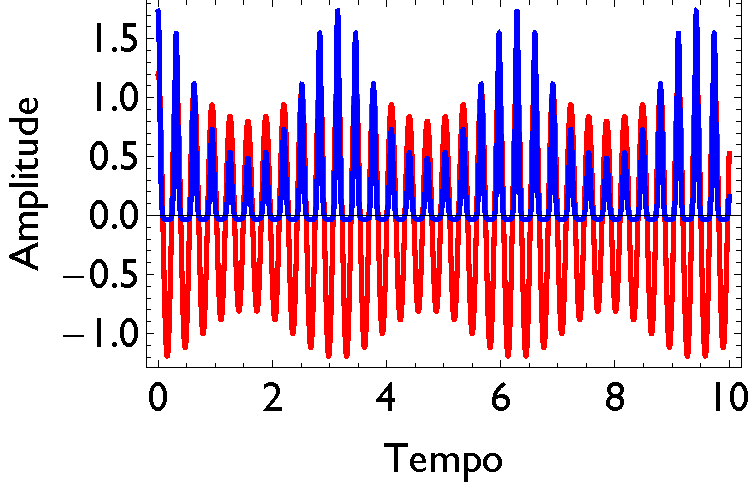
\includegraphics[width=0.3\textwidth]{diode_demodulation}
  \end{center}
   \vspace{-20pt}
  \caption{\textbf{Demodula��o por um diodo}}
\end{wrapfigure}

 Da mesma forma que modulamos a portadora para transmitir o sinal � necess�rio demodular a onda recebida para podermos escut�-la no alto-falante. Este � o papel do diodo neste circuito, devido a sua curva IV n�o-linear este componente recupera o sinal de audio que foi modulado na onda portadora.
 
\subsection*{Prepara��o}
\begin{enumerate}
\item Calcule a fun��o de trasfer�ncia $H(\omega)$ do filtro LC mostrado na figura \ref{fig:radio_am}. Mostre que a transmit�ncia ($|H|^2$) � dada por  $T(\omega)=\frac{L^2 \omega ^4 C_{in}^2}{\left(L \omega ^2 \left(C_{in}+C_v\right)-1\right){}^2}$. 
\item Qual � a frequ�ncia de resson�ncia deste filtro? 
\item Assumindo que o indutor possui $L=62\mu$H e o capacitor vari�vel pode variar entre $30\text{ pf}<C_v<350\text{ pf}$, calcule a faixa de frequ�ncias que este filtro poder� sintonizar. Descubra na internet quais r�dios de Campinas est�o nesta faixa.
\item Assuma que  a curva IV de um diodo pode ser aproximada pela express�o $i(t)=a_1 v(t)+a_2 v^2(t)$, onde $a_1$ e $a_2$ s�o constantes. Calcule a corrente quando a tens�o for na forma $v(t)=v_0(1+m(t))\cos[\omega_c t]$. Mostre que existe um termo proporcional � $m(t)$. Pense no  que acontece com os demais termos ao passar pelo capacitor do alto-falante?
\end{enumerate}
\subsection*{Material}
\begin{itemize}
\item Diodo de  sil�cio.
\item Diodo de germ�nio tipo Schotky (Nunca aplicar um sinal do gerador neste diodo, ele � sens�vel e pode queimar!).
\item Indutor e capacitor sintoniz�vel ( $30\text{ pf}<C_v<350\text{ pf}$) (Estes componentes j� est�o montados!).
\item Resistores: 1k $\Omega$.
\end{itemize}
\subsection*{Roteiro}
\subsubsection*{Caracteriza��o do circuito LC}
 \begin{wrapfigure}{r}{0.3\textwidth}
  \vspace{-30pt}
  \begin{center}
    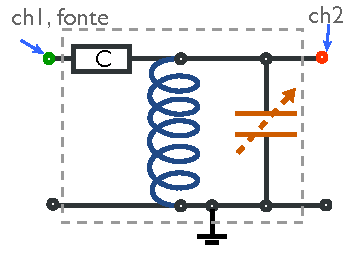
\includegraphics[width=0.3\textwidth]{tuning_lc}
  \end{center}
   \vspace{-20pt}
  \caption{\textbf{Esquema do circuito para caracterizar o filtro LC}. Utilize o gerador de fun��es no canal 1.}
  \label{fig:tuning}
\end{wrapfigure}
Para caracterizar o filtro iremos utilizar a montagem da Fig. \ref{fig:tuning}. Acople o sinal do gerador no terminal \textbf{verde} do filtro, me�a o sinal de sa�da no terminal \textbf{vermelho}. Estime a frequ�ncia de resson�ncia esperada e depois encontre-a experimentalmente para 4 diferentes posi��es das placas do capacitor sintoniz�vel. Com a maior capacit�ncia poss�vel, me�a 10 pontos das amplitudes $V_{pp1}/V_{pp2}$ na faixa de 50 KHz em torno da resson�ncia. No relat�rio estime a largura de banda do filtro.

\subsubsection*{Caracteriza��o da curva IV do diodo}

Em teoria poder�amos medir a curva IV de um diodo simplesmente introduzindo um resistor $R$ em s�rie com o diodo. A queda de tens�o  no resistor seria proporcional � corrente, portanto $I=V_R/R$. Para obter $V_D$ basta medirmos a queda de tens�o no diodo. Contudo, no  laborat�rio precisamos conectar o canal 1 do oscilosc�pio entre os terminais do diodo e o canal 2 entre os terminais de resistor. Como o terra de ambos canais � o mesmo, tal conex�o implicaria no resistor (ou o diodo)  em curto-circuito, portanto a queda de tens�o medida seria nula. Para resolver este problema de aterramento iremos explorar o transformador de tens�o pois neste o enrolamento prim�rio (conectado � rede el�trica) est� isolado do secund�rio (conectado ao circuito), consequentemente podemos impor um ponto de terra entre o resistor e o diodo, como ilustra a Fig. \ref{fig:diodo_iv}\footnote{Note que se fiz�ssemos esta conex�o utilizando o gerador sem o transformador, o resistor conectado ao terminal central do indutor estaria em curto-circuito.}. Como invertemos o sentido que estamos medindo a tens�o no resistor, � tamb�m necess�rio \textbf{inverter} o sinal do canal 2 do oscilosc�pio.

\begin{enumerate}
\item Monte o circuito da  Fig. \ref{fig:diodo_iv}.
\item No modo $YT$ do oscilosc�pio centralize ambas (canais 1 e 2) ondas em $Y=0$ e e grave no seu cart�o de mem�ria.
\item No modo $XY$ salve 2 vers�es da curva IV, uma em que a curva toda possa ser visualizada (ajuste as escalas horizontais e vertical) e outra em que a origem (pr�ximo de $V_R=0, V_D=0$) esteja ampliada.
\end{enumerate}

No seu relat�rio inclua as tr�s curvas. Para as curvas IV indique a escala vertical como corrente em mA e o eixo horizontal em V.
Extraia destas curvas a corrente de satura��o e tamb�m a inclina��o da curva $dI/dV$, para polariza��o reversa ($V<0$) e tr�s pontos distintos para polariza��o direta ($V>0$). Calcule a resist�ncia diferencial nestes pontos $R=(dI/dV)^{-1}$
 \begin{wrapfigure}{r}{0.5\textwidth}
  \vspace{0pt}
  \begin{center}
    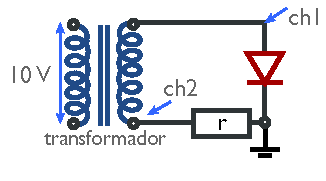
\includegraphics[width=0.5\textwidth]{diodo_iv}
  \end{center}
   \vspace{-20pt}
  \caption{\textbf{Esquema do circuito para caracterizar a curva IV}. Utilize o transformador de $9$ V de sa�da e $R=1K\Omega$ e um diodo de sil�cio \textbf{(encapsulamento preto!)}.}
  \label{fig:diodo_iv}
\end{wrapfigure}
\subsubsection*{Ouvindo o r�dio}
Chegou finalmente o momento de ouvirmos alguma m�sica (ou not�cias). Monte o circuito da Fig. \ref{fig:radio_am} utilizando como detetor o diodo schotky. A motivo de usarmos este diodo, ao inv�s do diodo de sil�cio,  � que a tens�o cr�tica na qual este diodo deixa passar corrente ($V_0\approx 30$ mV) � muito menor que o diodo de sil�cio ($V_0\approx 700$ mV). Isto o torna ideal para demodular sinais de pequena amplitude, como o que recebemos da antena. Muito cuidado com este diodo pois ele � sens�vel e n�o temos muitos sobrando. Descreva no relat�rio quais r�dios voc� consegui sintonizar. Em Campinas existem duas r�dios nesta faixa de frequ�ncias, a r�dio Central e a r�dio Bandeirantes

%----------------------------------

%AC


%%% Refer�ncias bibliog�ficas (geradas automaticamente)
%\addcontentsline{toc}{chapter}{Refer�ncias bibliogr�ficas}
%%\bibliographystyle{plainnat}  %% nome-ano
%\bibliographystyle{unsrt}    %% numero
%%%\bibliographystyle{osajnl}
%%%\bibliography{tese}
%\bibliography{references}

\end{document}

